% Chapter Template

\begin{savequote}[45mm]
The hair of the dog that bit you
\qauthor{Ancient proverb}
\end{savequote}

\chapter{Introduction: Carbon dioxide } % Main chapter title

\label{Chapter2} % Change X to a consecutive number; for referencing this chapter elsewhere, use \ref{ChapterX}

%----------------------------------------------------------------------------------------
%	SECTION 1
%----------------------------------------------------------------------------------------

\section{The chemical industry}

Industrialized societies depend on chemicals. In this discussion I define
chemicals as pure substances that are produced by industry for industry.
Chemicals might be used in the processing of products, or blended with other
chemicals in formulations that might be sold to users as products. As a familiar
example, sugar is produced by the sugar industry. It is a pure substance
(sucrose), and it is mostly used in the industry as an ingredient for processed
food: even the sugar that gets bought by consumers are not eaten raw but added
to food. \todo{Cite sugar uses}
 
The chemical industry produces a huge variety of products, anything from
something as simple as sulphuric acid to something as sophisticated as
medication. All of these chemicals help produce the products found necessary in
industrialized societies. Nevertheless, the chemical industry is not held in
high regard by people outside industry.\todo{cite perceptions of chemical industry}

A part of this negative perception comes from the chemical industry's reputation
for pollution. It pains me to say that this reputation is not undeserved. 

In 1984 a gas leak at a chemical plant in Bopal, India, caused the death of
thousands of people, and the injury of thousands more \todo{ citeBopal}. The ozone layer over
Antarctica is slowly recovering from depletion caused by the reckless emissions
of chlorofluorocarbons\todo{Cite ozone layer}. Plastics microparticles are now found everywhere in the
oceans \todo{autocite microplastics}, and the pesticide DDT is found in the breast milk of Inuit
mothers.\todo{autocite  DDT}

The chemical industry is also a prodigious producer of greenhouse gases. Apart
from the carbon dioxide emitted by the production of energy for chemical
processes, some chemical processes emit carbon dioxide as a waste product. One
of the most notable of these is the reduction of atmospheric nitrogen as the
first step in the production of nitrogen fertilizers. Of all the greenhouse
gases monitored by the IPCC, only carbon dioxide, methane and nitrous oxide are
found in nature: the others are exclusively products of the chemical industry.\todo{autocite{AR4 } }

While it is true that these impacts were caused by human negligence or
ignorance, and not by the chemicals themselves, which are well-behaved when they
are used in controlled environments, the moral response must be to look at the
intrinsic safety of chemicals.
 
%-----------------------------------
%	SUBSECTION 1
%-----------------------------------
\subsection{``Green chemistry''}

The date of the birth environmental movement is conventionally set to 1962, when
the biologist Rachel Carson published the book \textit{Silent Spring}, which
pointed out the destruction of nature by the unrestricted use of pesticides, and
the dangers of overuse. This was a direct imputation of the chemical industry,
because the pesticide products contained many chemicals. 

Chemists are human, and the realization that chemicals can have detrimental
effects brought at least some chemists to reflect on their own work. This has
given rise to the concept of \textit{green chemistry}. Although the term has no
rigorous definition or quantitative measure\autocite{Linthorst2010}, a set of 12
principles or guidelines are proposed:

\begin{enumerate}
  \item It is better to prevent waste than to treat or clean up waste after it is formed.
  
  \item Synthetic methods should be designed to maximize the incorporation of
  all materials used in the process into the final product.
  
  \item Wherever practicable, synthetic methodologies should be designed to use
  and generate substances that possess little or no toxicity to human health and
  the environment.
  
  \item Chemical products should be designed to preserve efficacy of function
  while reducing toxicity.
  
  \item The use of auxiliary substances (e.g. solvents, separation agents, etc.)
  should be made unnecessary wherever possible and innocuous when used.
  
  \item Energy requirements should be recognized for their environmental and
  economic impacts and should be minimized. Synthetic methods should be
  conducted at ambient temperature and pressure.
  
  \item \label{itm:renewable}A raw material or feedstock should be renewable
  rather than depleting wherever technically and economically practicable.
  
  \item Unnecessary derivatization (blocking group, protection/deprotection,
  temporary modification of physical/chemical processes) should be avoided
  whenever possible.
  
  \item Catalytic reagents (as selective as possible) are superior to
  stoichiometric reagents.
  
  \item Chemical products should be designed so that at the end of their
  function they do not persist in the environment and break down into innocuous
  degradation products.
  
  \item Analytical methodologies need to be further developed to allow for
  real-time, in process monitoring and control prior to the formation of
  hazardous substances.
  
  \item Substances and the form of a substance used in a chemical process should
  be chosen so as to minimize the potential for chemical accidents, including
  releases, explosions, and fires.

\end{enumerate}

While these guidelines are clearly written with synthetic chemistry in mind, it
does not mean that they do not apply to analytical chemistry. Item
\ref{itm:renewable} suggests that, when possible, one should use hydrogen rather
than helium as mobile phase in capillary gas chromatography: hydrogen is
renewable, whereas there is only a finite amount of helium available. 

One large area of the greening of chemistry is changing the use of solvents.
Solvents play a large role in everyday chemistry, but most solvents used in
chemistry are ultimately derived from petroleum, and most are toxic to some
degree.

One application for solvents is extractions. Extractions can be either from a
solid material, as in extracting aspirin from willow bark, or liquid-liquid,
where a compound is extracted from one liquid into another. 

A good bit of work is being done to create new solvents to replace existing
ones.\todo{autocite new green solvents} But there are a few solvents that are
already ``green'', such as water or ethanol.

One such naturally green solvent is carbon dioxide. 
 
% ----------------------------------- SUBSECTION 2
% -----------------------------------

\subsection{Carbon dioxide as a green chemical}

Carbon dioxide as a chemical is used in industry in a few key areas.

\begin{itemize}
  
  \item Carbon dioxide is often used in firefighting, in the form of portable
  fire extinguishers, or room flooding systems. In this last use it is
  displacing the ozone-depleting halomethane (Halon).
  
  \item When liquid water is supersaturated with carbon dioxide, the gas
  escapes slowly in the form of streams of tiny bubbles. This phenomenon makes
  beverages prepared from water supersaturated with carbon dioxide (or
  \textit{carbonated water}) interesting to drink, and a large, international
  industry is based on carbonated water.
   
   \item Carbon dioxide has a freezing point of {-}77 °C, and the solid can be
   conveniently obtained by evaporating liquid carbon dioxide at atmospheric
   pressure. The evaporating liquid rapidly cools the stream of carbon dioxide,
   lowering the temperature of the stream to below the freezing point, and the
   gas crystallizes into the solid. The resulting `snow' can be compressed into
   blocks, which only slowly sublimates into gaseous carbon dioxide. Packing
   frozen food products together with this 'dry ice' allows for it to be
   transported cold, 
   
   \item Pellets of dry ice can be entrained in a jet of air, and used to abrade
   surface for cleaning \autocite{Spur1999}. This use of carbon dioxide can
   displace toxic solvents and/or abrasives dust.
   
   \item Carbon dioxide is a `natural refrigerant' \autocite{Pearson2005}, and
   can be used to displace hydrofluorocarbon refrigerants, which are potent,
   long-lived greenhouse gases.
   
   \item Carbon dioxide can be used as a preservative and anti-oxidant in
   packaged food. If headspace air in a packaged food is removed by purging it
   with carbon dioxide, the growth of microbes can be discouraged, extending the
   shelf life of the product \autocite{Jacobsen2002}.
	   
	\item Carbon dioxide can be used to extract compounds from natural products. 
	
\end{itemize}

%----------------------------------------------------------------------------------------
%	SECTION 2
%----------------------------------------------------------------------------------------

Of these uses, extractions are economically the most important.

\section{Extractions using carbon dioxide}

\subsection{Commercial extractions}

There are several commercial processes that use

\subsubsection{Plant oils}

Vegetable oils are obtained from various crops, and are can be extracted from
the substrate by pressing, heating or extraction. High-pressure carbon dioxide
has been used to extract vegetable oils. 

\subsubsection{Hops}

Hops is an essential component in the brewing of beer. It imparts a desired
bitter flavour, stabilizes the beer during storage, and assists with foam
formation \autocite{Schoenberger2011}. Hops is a seasonal crop with a limited
growing range, but the demand for beer is not limited to certain areas or
seasons. The creation of hops extract makes it possible to have the benefit of
hops without owning a hops plantation or storing and transporting dried hops
over long distances. All hops extracts produced today are extracted by carbon dioxide \autocite{Hunt2010}. 

\subsubsection{Coffee}

Coffee is an international industry, with coffee drunk in many cultures and in
many forms. One of the attractions of coffee is the effects of the psychoactive
substance, caffeine. Caffeine is a mild stimulant and promotes wakefulness. A
small proportion of coffee drinkers enjoy drinking coffee, but prefer to avoid
the stimulant effect, which might induce insomnia. For these coffee drinkers the
market supplies decaffeinated coffee. 

Given the large amount of coffee traded (an estimated 167.47 million bags of
coffee in the 2018-2019 coffee year \autocite{Coffee2018})\footnote{The factoid
that ``coffee is the second-most traded commodity after oil'' has been proven to
be untrue.\autocite{Greenberg2017}}, if only a small percentage of coffee needs
to be decaffeinated, it will be a large amount of coffee to process, and
industrial processes will be necessary to supply the demand.

Decaffeination of coffee is achieved by selectively extracting the caffeine from
green (\textit{i.e.} unroasted) coffee beans using carbon dioxide. This is the
largest use of carbon dioxide for extraction \autocite{Ramalakshmi1999}. The
extracted caffeine is sold for use in medication and cold drinks. 

\subsection{Analytical Extractions}

The first extractions using carbon dioxide was of course not aimed at developing
an industrial operation, but to develop a method for analytical chemistry. This
method is usually called SFE, for \textbf{s}upercritical \textbf{f}luid
\textbf{e}xtraction.

\subsection{Why carbon dioxde?}

But what makes it better than any other solvent?

There are two aspect to this question. The first is about the \textit{greenness}
of carbon dioxide. It is non-toxic, non-persistent, non-flammable,
non-corrosive, inexpensive, commercially available, and a waste product. (It
goes without saying that this carbon dioxide is sourced from a carbon-neutral
source, perhaps the brewery industry.)

The second aspect of the desirability of carbon dioxide lies in its physical
properties and the conditions under which we use it. 

Chemists will intuitively understand that gaseous carbon dioxide has no solvating
properties, and that liquid carbon dioxide should not behave much differently
than any other solvent. Both these statements are true under 'normal' circumstances.

Consider the case of an isobaric cooling of a volume of gas.The gas-liquid
transition takes place because energy is removed from the system.
At some point the kinetic energy of some of the molecules becomes less than the
energy of the intermolecular forces, and the molecules prefer to clump together.
The remaining gas molecules receive the excess energy, and therefore stay in the
gas state, until more energy is removed.

Now consider a solute (solid or liquid) in the same volume of gas being cooled.
In this case, as the gas cools the gas-solute intermolecular forces can become
more important in the gas-gas interaction at a temperature which is higher than
the boiling point. In such a case the gas will have solvating properties, and
the solute will become truly dissolved in the gas.

The same argument follows during the isothermal compression of a gas. 

If there are more than one solute in the volume of gas, some might dissolve in
the gas, while others one might not. This means that the solvating gas can be
\textit{selective}. It can also be seen that the solvating power of the gas will
depend on the temperature and the pressure of the gas. This means that the
solvent becomes \textit{tunable}.

While the compressed gas has solvating properties, it still has the physical
properties of a gas:

\begin{description} 

\item[Diffusivity] The solvating gas maintains its low diffusion coefficient,
which means that it can easily diffuse into porous material, and that solutes
will rapidly diffuse through it. \done \todo{diffusivity of CO2}

\item[Surface tension] The solvating gas has a low surface tension, which means
that it will readily `wet' surfaces and penetrate porous material. \done \todo{surface tension of CO2}

\item[Viscosity] The solvating gas has a low viscosity, which means that it
takes little energy to pump it. \done \todo{viscosity of CO2}

\end{description} 

For historical reasons, such solvating gases are known as a 'supercritical
fluids', because they are usually obtained by heating a liquid at high pressure,
so that the temperature and pressure of the substance is higher than it's
\textit{critical point}. The critical pressure of a substance is the pressure
above which it is impossible to create a gas-liquid phase transition by isobaric
cooling, and the critical temperature is the temperature above which it is
impossible to create a gas-liquid phase transition by isothermal compression.
When the gas is at its critical temperature and critical pressure, it is at its
critical point. The critical point is very different from the \textit{triple
point}: there is no equilibrium involved. (See figure \ref{fig:co2phase}.) The
terms `supercritical fluid' and `dense gas' are synonymous --- the term 'dense
gas' of course implies that the gas behaviour is far from that of an ideal gas.

\begin{todo} 
In practice, near the critical point there are only very small differences
between the properties of the liquid and the gas, so that many separations that
are done below supercritical temperature but at high pressure.
\end{todo}

\begin{figure}
\centering
\includegraphics[width=\textwidth]{Figures/CO2PhaseDiagram}
\decoRule
\caption[The carbon dioxide phase diagram]{The phase diagram of carbon dioxide}
\label{fig:co2phase}
\end{figure}

The critical pressure of carbon dioxide is 304.12 K (31.10 °C) , and the,
critical pressure is 7.39 MPa (72.9 atm). This temperature and pressure are easy
to achieve in the laboratory with standard chromatographic instrumentation, or
indeed in an industrial plant with using process engineering technologies.

Carbon dioxide is gaseous at ambient conditions. This means that once it has
been used in it's role as extractant, and it is exposed to the atmosphere, it
will rapidly evaporate, without needing added heat, and leaving no residues.

The practical alternatives to carbon dioxide as a supercritical fluid are
ammonia, methanol, CFCs/Freon, hydrocarbons (propane, butane), water and sulfur
hexafluoride. All of these lack green attributes: hyrocarbons pollute, the CFCs
deplete ozone, sulfur hexafluoride is a potent greenhouse gas, and methanol and
water are liquid at ambient conditions.

For these reasons the term supercritical fluid is practically synonymous with
high-pressure carbon dioxide .

It is also possible to use supercritical fluids as . This topic
falls outside the scope of this discussion.
 
\subsubsection{Modifiers}

While the solvating power of a supercritical fluid is certainly `tuneable' by
adjusting its pressure and/or temperature, the range in solubility might be
quite limited in practice. Supercritical carbon dioxide is quite non-polar, with
a polarity ascribed to it similar to that of dichloromethane, although the
reality is more complex. \todo{autocite CO2 polarity paper.}

Just as with other solvents, it is possible to add a co-solvent or
\textit{modifier} to the supercritical carbon dioxide. This makes it possible to
increase the solubility of polar compounds in the supercritical fluid. Methanol,
ethanol, formic acid and water are examples of suitable green modifiers for
carbon dioxide.

When modifiers are used the carbon-dioxide, modifier and solute forms a system
with four degrees of freedom (modifier percentage, solute concentration,
pressure, and temperature), which can become difficult to model. While this is a
challenge for process engineers who need to design efficient industrial systems,
analytical chemists can afford to be pragmatic and use heuristics to find
suitable conditions.

\subsubsection{Practical extractions}

Figure \ref{fig:sfediagram} shows a schematic diagram of a system set up for supercritical fluid extractions. 

\begin{figure}
\centering
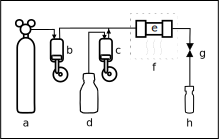
\includegraphics[width=\textwidth]{Figures/SFE_System}
\decoRule

\caption[SFE system diagram]{A diagram of an SFE system. (a) CO\textsubscript{2} supply (b)
High-pressure SF pump (c) High-pressure modifier pump (d) Modifier reservoir (e)
Extraction cell (f) Pressure control (g) Collection vessel}

\label{fig:sfediagram}
\end{figure}

\todo{Add dip tube to CO\textsubscript{2} cylinder}
\todo{Add heater to extraction cell}

Carbon dioxide (a) is readily available from suppliers of industrial gases, and
high-purity grades are available. Chromatography-grade solvents are usually used
as modifiers (d). High-pressure pumps (HPLC type) are used to compress the
carbon dioxide (b) and the modifier (c), which are mixed together at the
appropriate ratio. The mixture gets pumped into the (optionally heated (f))
extraction cell (e), which contains the material that needs to be extracted.
Having extracted the extract from the material, the supercritical fluid passes
through a pressure-control mechanism (g). This allows the pressure of the
supercritical fluid to drop to ambient, turning it into a low-density
non-solvating gas. The extract becomes desolvated, and precipitates in the
collection vessel (h). The operation of the system might be either static or
dynamic: in static operation the supercritical fluid is pumped into the system,
the flow is stopped, and the matrix/fluid mixture is given time to approach
equilibrium. Then the fluid is expelled and the extract collected.
In dynamic operation the supercritical fluid is pumped through the extraction
cell and the extract collected continuously. 


\section{Supercritical Fluid Chromatography}

An analyte will extract out of a matrix with a certain efficiency and at a
certain rate. While this is important while finding an optimum extraction
method, otherwise its relevance is limited.

However, different analytes will extract out of a matrix with different
efficiency and at different rates. In 1903 the Russian botanist Tsvet
\todo{autocite Tsvett} applied this observation to the dynamic extraction of a
bed of calcium carbonate that had an extract of plant pigments applied at the
inlet end. The different extraction efficiencies and rates of adsorption and
desorption on the calcium carbonate surface lead to the \textit{separation} of
the compounds in the mixture. Tsvet called this method of separation
\textit{chromatography}. With time this method became generalized, and today
chromatography is a major, established scientific field with many ramifications
and a myriad of applications.

Because of the different technologies used in its applications, chromatography
is conventionally classed as either \textit{gas chromatography} (GC) or
\textit{liquid chromatography} (LC). However, as we have seen, solvating gases
can also extract analytes from solid stationary phases, and hence the therm
\textit{supercritical fluid chromatography} (SFC) was created for these kind of
separations. 

Supercritical fluid chromatography as practised today bears a lot of resemblance
to \textit{high performance liquid chromatography} (HPLC). The main reason for
this is that there is a large overlap between the technology used for HPLC and
the technology needed for SFC. In particular, both use high-pressure pumps and
columns packed with particles with very small diameter, and use optical
detectors. The same instrument manufacturers who supply HPLC instrumentation
also supply SFC instrumentation.

\todo{ELSD}

\subsection{SFC and FID}

Did not always But this was not always so. In the 1980s SFC was practised using open tubular
columns and FID detectors, so the instrument designs looked more like GC instruments than HPLC instruments. 

The \textit{flame ionization detector} was invented near-simultaneously in South
Africa and New Zealand \todo{autocite FID history}. The core of the system is a
flame of hydrogen gas burning in air. The measured signal is the conductivity of
the flame plasma, which is measured by applying a -100 V potential difference
between electrodes at the tip and the base of the flame. There are very few free
ions in the hydrogen flame, so the conductivity is normally low. But organic
compounds introduced into the flame creates a number of free ions, which
increases the conductivity of the flame gases. The change in conductivity is
measured by measuring the current between the two electrodes, using an electrometer. 

The carbon dioxide in an SFC detector 

\todo{FID diagram}

The FID is quite sensitive: an x \% change in concentration will give a y \%
change in signal. This is similar to the UV detector, in which the molar
absorptivity determines the detector response. Where the FID outshines any
optical detector is in its dynamic range. The UV detector has \textit{dynamic
range} of 1000, \textit{i.e.} it can detect a 1000-fold change in concentration,
but the dynamic range of the FID detector is unsurpassed at 1000 000. This makes
the FID an excellent detector if quantitation needs to be done.

During the time SFC looked like GC, the FID was the detector of choice. But when SFC
started looking like HPLC, and the selectivity of the chromatography started
being manipulated by adding modifiers, the FID lost its utility. The quantity of modifier added to the carbon

\todos